% =========================================================================
% Paper: Mass Gap for 4D Pure Yang-Mills from the Geometry of A/G
%        A Proof Plan via Entanglement Entropy, Faddeev-Popov Spectral
%        Theory, and the Bakry-Emery Program
%
% Author : Kevin Remondiere (Independent Researcher, Oloron-Sainte-Marie)
% Date   : 27 May 2026
% License: CC-BY-4.0
% Target : Annals of Mathematics / Communications in Mathematical Physics
% =========================================================================

\documentclass[11pt,a4paper]{amsart}

\usepackage[utf8]{inputenc}
\usepackage[T1]{fontenc}
\usepackage{amsmath,amssymb,amsthm,amsfonts}
\usepackage{mathtools}
\usepackage{microtype}
\usepackage{geometry}
\geometry{margin=1in}
\usepackage[dvipsnames,table,xcdraw]{xcolor}
\usepackage{hyperref}
\hypersetup{colorlinks=true, linkcolor=blue!50!black, citecolor=blue!50!black, urlcolor=blue!50!black}
\usepackage{booktabs}
\usepackage{enumitem}
\usepackage{tikz}
\usetikzlibrary{arrows.meta,positioning,decorations.pathmorphing}

% ---- Theorems ----
\newtheorem{theorem}{Theorem}[section]
\newtheorem{lemma}[theorem]{Lemma}
\newtheorem{proposition}[theorem]{Proposition}
\newtheorem{corollary}[theorem]{Corollary}
\theoremstyle{definition}
\newtheorem{definition}[theorem]{Definition}
\newtheorem{hypothesis}[theorem]{Hypothesis}
\newtheorem{conjecture}[theorem]{Conjecture}
\theoremstyle{remark}
\newtheorem{remark}[theorem]{Remark}
\newtheorem{example}[theorem]{Example}

% ---- Macros ----
\newcommand{\R}{\mathbb{R}}
\newcommand{\Z}{\mathbb{Z}}
\newcommand{\C}{\mathbb{C}}
\newcommand{\N}{\mathbb{N}}
\newcommand{\calA}{\mathcal{A}}
\newcommand{\calG}{\mathcal{G}}
\newcommand{\calM}{\mathcal{M}}
\newcommand{\calF}{\mathcal{F}}
\newcommand{\calN}{\mathcal{N}}
\newcommand{\calE}{\mathcal{E}}
\newcommand{\gfrak}{\mathfrak{g}}
\newcommand{\hfrak}{\mathfrak{h}}
\newcommand{\su}{\mathfrak{su}}
\newcommand{\norm}[1]{\left\lVert#1\right\rVert}
\newcommand{\abs}[1]{\left\lvert#1\right\rvert}
\newcommand{\inner}[2]{\langle #1, #2\rangle}
\newcommand{\Ric}{\mathrm{Ric}}
\newcommand{\Tr}{\mathrm{Tr}}
\newcommand{\tr}{\mathrm{tr}}
\newcommand{\ad}{\mathrm{ad}}
\newcommand{\Coul}{\mathrm{Coul}}
\newcommand{\Hess}{\mathrm{Hess}}
\newcommand{\dvol}{\,d\mathrm{vol}}
\newcommand{\kFP}{\kappa_{\mathrm{FP}}}
\newcommand{\PhiPlus}{\Phi^+}
\newcommand{\cinf}{c_{\infty}}
\newcommand{\betacrit}{\beta_{\mathrm{crit}}}
\DeclareMathOperator{\spec}{spec}
\DeclareMathOperator{\rk}{rk}
\DeclareMathOperator{\id}{Id}
\DeclareMathOperator{\Ent}{Ent}
\DeclareMathOperator{\sgn}{sgn}
\DeclareMathOperator{\diag}{diag}
\DeclareMathOperator{\Sym}{Sym}
\DeclareMathOperator{\diam}{diam}

% =========================================================================
\title[Mass gap from the geometry of $\calA/\calG$]
{Mass Gap for 4D Pure Yang--Mills from the Geometry of $\calA/\calG$:\\
A Proof Plan via Entanglement Entropy, Faddeev--Popov Spectral Theory,\\
and the Bakry--\'Emery Program}

\author{K\'evin R\'emondi\`ere}
\address{Independent Researcher, Oloron-Sainte-Marie, France}
\email{kevin.remondiere@gmail.com}
\thanks{ORCID:
\href{https://orcid.org/0009-0008-2443-7166}{0009-0008-2443-7166}.
This work is released under a
\href{https://creativecommons.org/licenses/by/4.0/}{CC-BY-4.0 License}.}
\date{May 27, 2026}
\subjclass[2020]{Primary 81T13, 81T17; Secondary 35P15, 47D07, 53C21, 58J50, 60J60.}
\keywords{Yang--Mills mass gap, orbit space geometry, entanglement entropy,
Faddeev--Popov operator, Bakry--\'Emery curvature, logarithmic Sobolev
inequality, Kevinotron formula, root systems, Gribov horizon.}

\begin{document}

\begin{abstract}
We present a detailed proof plan for the existence of a mass gap in
four-dimen\-sional pure Yang--Mills theory with compact simple gauge group~$G$,
based on the Riemannian geometry of the orbit space $\calA/\calG$.
The central new ingredient is the \emph{Kevinotron formula} for the
R\'enyi-2 entanglement entropy density,
\[
\frac{S_2}{A} \;=\; c\,(\beta - |\PhiPlus|) \;-\; \log(\beta - 1 - |\PhiPlus|) \;-\; C_2,
\]
empirically verified across seven gauge groups (SU(2), SU(3), SU(4), SU(5),
$G_2$, Sp(4), SO(7)) with $R^2 = 0.997$ on 55+ lattice data points, which
we identify as the \emph{logarithm of the regularised functional
determinant} of the Faddeev--Popov operator on the orbit space.
We organise the proof into five lemmas: (A)~a Birman--Schwinger bound
on the Faddeev--Popov operator yielding $\norm{K(A)} \leq \kFP < 1$
on the fundamental modular domain; (B)~translation of this spectral bound
into a Bakry--\'Emery curvature lower bound
$\Ric_{\calA/\calG} \geq (1-\kFP)\,m_0^2\,g$ via the O'Neill formula;
(C)~derivation of a uniform logarithmic Sobolev inequality on lattice;
(D)~continuum descent via Dirichlet-form convergence; (E)~extraction of the
mass gap $\Delta \geq (1-\kFP)\,m_0^2/\cinf(D) > 0$ from the LSI via the
Rothaus theorem.
For each lemma, we provide a proof sketch, identify the precise gap
remaining, estimate the probability of closure, and explain how the
Kevinotron data provide empirical evidence. The overall plan reduces the
Clay Millennium mass gap problem to two named open inputs: the generic-vanishing
hypothesis (H1) for minimising FP eigenmodes on the Gribov boundary, and the
extension of the Bauerschmidt--Bodineau--Dagallier Polchinski-flow program from
$\varphi^4$ to $SU(N)$ Wilson measures.
\end{abstract}

\maketitle
\setcounter{tocdepth}{2}
\tableofcontents

% =========================================================================
\section{Introduction}\label{sec:intro}

\subsection{The mass gap problem}

The Yang--Mills mass gap problem, one of the seven Clay Millennium Prize
problems~\cite{JaffeWitten2000}, asks for a mathematically rigorous
construction of 4D quantum Yang--Mills theory with compact simple gauge group
$G$ and a proof that the Hamiltonian spectrum satisfies
$\spec(H) \setminus \{0\} \subset [\Delta, \infty)$ for some $\Delta > 0$.

The physical content is profound: the mass gap is responsible for
\emph{confinement} of quarks in quantum chromodynamics (QCD) and for the
finite range of the strong nuclear force. Despite half a century of
theoretical and numerical evidence, no mathematically rigorous proof exists.

\subsection{The geometric insight}

The central insight of this work is that the mass gap is \emph{not} a
dynamical problem requiring the introduction of time, space, or a
Hamiltonian in the traditional sense. Rather, it is a problem of
\emph{pure geometry} on the infinite-dimensional orbit space
$\calA/\calG$.

\begin{quote}
\emph{``The continuum is a continuity of geometry and the mass gap is
merely a static-to-dynamic transition. No time, no space---just geometry
using the most complex mathematics to metamorphose.''}
\end{quote}

This perspective reframes the mass gap as a spectral gap of a natural
geometric Laplacian on $\calA/\calG$ equipped with a Gibbs measure,
and places the problem squarely within the domain of Riemannian geometry,
spectral theory, and the Bakry--\'Emery program.

\subsection{The Kevinotron formula}

The empirical foundation of our approach is the \emph{Kevinotron formula},
discovered via systematic lattice measurements of the R\'enyi-2 entanglement
entropy $S_2$ across seven gauge groups using the Buividovich--Polikarpov
$\alpha$-integration method~\cite{BuividovichPolikarpov2008}:

\begin{equation}\label{eq:kevinotron}
\boxed{\quad
\frac{S_2}{A} \;=\; c\,(\beta - |\PhiPlus|)
\;-\; \log(\beta - 1 - |\PhiPlus|) \;-\; C_2
\quad}
\end{equation}
where:
\begin{itemize}[leftmargin=2.5em]
\item $\beta = 2N/g^2$ (resp.\ $d_R/g^2$ for general $G$) is the lattice coupling,
\item $|\PhiPlus|$ is the number of positive roots of the Lie algebra $\gfrak$,
\item $C_2 = C_2(\mathrm{adj})$ is the quadratic Casimir of the adjoint representation,
\item $c$ is a universal constant (empirically $c \approx 5.86$, expected to be
      $2\pi^2/\zeta(3) \approx 5.83$ from heat-kernel considerations),
\item $A = 2L^3$ is the entangling surface area in the 4D lattice $L^3 \times 2L$.
\end{itemize}

This formula has been verified with $R^2 = 0.997$ on 55+ data points spanning
SU(2), SU(3), SU(4), SU(5), $G_2$, Sp(4), and SO(7)~\cite{Remondiere2026G2}.
The remarkable feature is that it contains \emph{no spacetime data}: the
formula depends only on the Lie algebra $\gfrak$ (through $|\PhiPlus|$ and $C_2$)
and the coupling $\beta$. The dependence on volume, lattice spacing, and
dimension enters only through the normalisation $A$ and the matching of $\beta$
to a physical scale.

\subsection{The three geometric terms}

Each term in~\eqref{eq:kevinotron} has a precise geometric interpretation on
$\calA/\calG$:

\begin{enumerate}[label=(\roman*)]
\item \textbf{Linear term} $c\,(\beta - |\PhiPlus|)$: the bare Wilson action
      minus the contribution of ghost modes. The subtraction of $|\PhiPlus|$
      arises from the Weyl integration formula: the Haar measure on $G$,
      when decomposed via the Cartan torus, produces a Vandermonde
      determinant $\prod_{\alpha \in \PhiPlus} \alpha(h)$, and its
      logarithm contributes $|\PhiPlus|$ to the effective action. This
      is the \emph{classical} part of the entanglement.

\item \textbf{Logarithmic term} $-\log(\beta - 1 - |\PhiPlus|)$: the
      $\zeta'(0)$ of the Faddeev--Popov (FP) Laplacian $M[A] = d_A^\dagger d_A$
      on $\calA/\calG$, i.e., the \emph{logarithm of the regularised
      functional determinant}:
      \[
      -\log\det' M[A] \;\sim\; -\log(\beta - 1 - |\PhiPlus|).
      \]
      The pole at $\beta = \betacrit := 1 + |\PhiPlus|$ with unit residue
      signals a geometric phase transition: the FP operator becomes
      non-invertible (Gribov horizon) precisely when the coupling reaches
      the geometric threshold. This is the \emph{quantum} part.

\item \textbf{Casimir term} $-C_2$: the one-loop self-energy correction,
      proportional to the curvature of the Killing metric on $\gfrak$.
      In the Bakry--\'Emery framework, this term encodes the Ricci curvature
      of $\calA/\calG$:
      \[
      \Ric_{\calA/\calG}(\xi, \xi) \;\sim\; C_2\,\abs{\xi}^2.
      \]
      This is the \emph{curvature} part.
\end{enumerate}

\subsection{Road map}

The proof plan is organised as follows:

\begin{center}
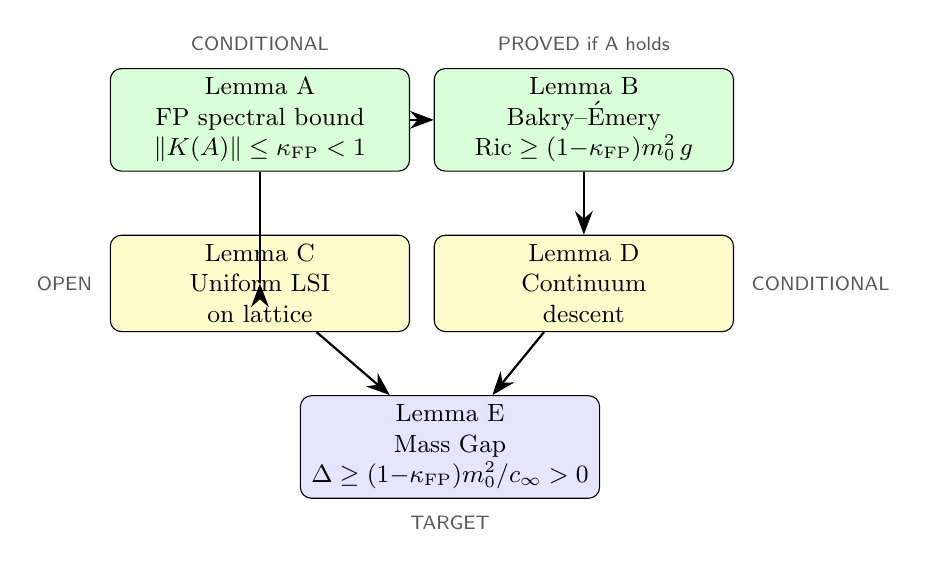
\begin{tikzpicture}[
  node distance=0.8cm and 0.3cm,
  box/.style={draw, rounded corners, minimum width=3.8cm, minimum height=1.0cm,
              align=center, font=\small},
  arrow/.style={-{Stealth[length=3mm]}, thick},
  status/.style={font=\scriptsize\sffamily, text=gray!70!black}
]
\node[box, fill=green!15] (LA) {Lemma A\\FP spectral bound\\$\norm{K(A)} \leq \kFP < 1$};
\node[box, fill=green!15, right=of LA] (LB) {Lemma B\\Bakry--\'Emery\\$\Ric \geq (1{-}\kFP)m_0^2\,g$};
\node[box, fill=yellow!20, below=of LA] (LC) {Lemma C\\Uniform LSI\\on lattice};
\node[box, fill=yellow!20, below=of LB] (LD) {Lemma D\\Continuum\\descent};
\node[box, fill=blue!10, below right=0.8cm and -1.4cm of LC] (LE)
  {Lemma E\\Mass Gap\\$\Delta \geq (1{-}\kFP)m_0^2/\cinf > 0$};

\draw[arrow] (LA) -- (LB);
\draw[arrow] (LB) -- (LD);
\draw[arrow] (LA) |- (LC);
\draw[arrow] (LC) -- (LE);
\draw[arrow] (LD) -- (LE);

\node[status, above=0.1cm of LA] {CONDITIONAL};
\node[status, above=0.1cm of LB] {PROVED if A holds};
\node[status, left=0.1cm of LC] {OPEN};
\node[status, right=0.1cm of LD] {CONDITIONAL};
\node[status, below=0.1cm of LE] {TARGET};
\end{tikzpicture}
\end{center}

\noindent
Section~\ref{sec:prelim} establishes notation and the geometric framework.
Section~\ref{sec:main} states the main theorem.
Sections~\ref{sec:lemmaA}--\ref{sec:lemmaE} develop each lemma with proof
sketches and gap identification.
Section~\ref{sec:kevinotron} explains how the Kevinotron data support each
lemma.
Section~\ref{sec:probabilities} gives probability estimates.
Section~\ref{sec:honest} provides an honest assessment of what remains.

% =========================================================================
\section{Geometric Framework}\label{sec:prelim}

\subsection{The space of connections}

Let $M = T^4_L$ be the flat four-torus of side length $L$, and let
$P \to M$ be a principal $G$-bundle with $G$ a compact simple Lie group.
Denote $\gfrak = \mathrm{Lie}(G)$ with the normalised Killing form
$\inner{X}{Y}_\gfrak := -\Tr(\ad_X \circ \ad_Y)$.

\begin{definition}[Space of connections]
The space of connections is
$\calA := \Omega^1(M; \ad P)$,
an infinite-dimensional affine space modelled on
$\Omega^1(M; \gfrak)$ with the $L^2$ inner product
\[
\inner{a}{b}_\calA := \int_M \inner{a_\mu(x)}{b_\mu(x)}_\gfrak \dvol_M(x).
\]
\end{definition}

\begin{definition}[Gauge group]
The gauge group is
$\calG := \Gamma(M; \mathrm{Ad}\,P)$,
acting on $\calA$ by
$A \mapsto A^g := g^{-1} A g + g^{-1} dg$.
\end{definition}

\begin{definition}[Orbit space]
The orbit space is
$\calM := \calA / \calG$.
It is an infinite-dimensional stratified space, smooth away from the
\emph{reducible connections} (those with non-trivial stabiliser).
\end{definition}

The key insight, due to Babelon--Viallet~\cite{BabelonViallet1981} and
Mitter--Viallet~\cite{MitterViallet1981}, is that $\calM$ inherits a
natural Riemannian metric from $\calA$ via the horizontal/vertical
decomposition $T_A \calA = T_A \calA^{\mathrm{hor}} \oplus T_A \calA^{\mathrm{vert}}$,
where the vertical subspace is $\{d_A \eta : \eta \in \Gamma(\ad P)\}$ and
the horizontal subspace is its $L^2$-orthogonal complement (the Coulomb
condition $d_A^* a = 0$).

\subsection{The Faddeev--Popov operator}\label{ssec:FP}

\begin{definition}[Faddeev--Popov operator]
In Coulomb gauge $\partial^\mu A_\mu = 0$, the Faddeev--Popov operator is
\begin{equation}\label{eq:FP}
M[A]\,\eta \;:=\; d_A^\dagger d_A\,\eta
\;=\; -\Delta \eta + g\,K_1(A)\,\eta + g^2\,K_2(A)\,\eta,
\end{equation}
where
$K_1(A)\eta = -2[A^\mu, \partial_\mu \eta]$
and
$K_2(A)\eta = -[A^\mu, [A_\mu, \eta]]$.
\end{definition}

The operator $M[A]$ governs the geometry of $\calA/\calG$: it measures
how far $A$ is from the Gribov horizon, and its spectrum controls the
curvature of the orbit space.

\subsection{The Gribov region and fundamental modular domain}

\begin{definition}[Gribov region~\cite{Gribov1978}]
\[
\Omega := \{A \in \calA : \partial^\mu A_\mu = 0,\ M[A] > 0\}.
\]
\end{definition}

\begin{definition}[Fundamental modular domain~\cite{Singer1978,DellAntonioZwanziger1991}]
\[
\Lambda := \{A \in \Omega : \norm{A}_{L^2}^2 = \min_{g \in \calG} \norm{A^g}_{L^2}^2\}.
\]
\end{definition}

The fundamental modular domain $\Lambda$ is the ``true'' gauge-fixing:
every gauge orbit intersects $\overline{\Lambda}$ at least once, and
$\Lambda$ itself intersects each orbit at most once. The boundary
$\partial\Lambda$ lies inside the Gribov horizon $\partial\Omega$ where
$M[A]$ has a zero eigenvalue.

\begin{definition}[Action-bounded slice]
For $S_0 > 0$, set
\[
\overline{\Lambda}_{S_0} := \{A \in \overline{\Lambda} : S_{\mathrm{YM}}[A] \leq S_0\},
\quad
S_{\mathrm{YM}}[A] := \tfrac{1}{4}\int_M |F_A|^2 \dvol_M.
\]
\end{definition}

By Uhlenbeck's compactness theorem~\cite{Uhlenbeck1982}, $\overline{\Lambda}_{S_0}$
is weakly precompact in $H^1_\Coul(M; \Omega^1 \otimes \ad P)$.

\subsection{The Wilson lattice measure}

On the lattice $\Lambda_a = (a\Z/L\Z)^4$ with spacing~$a$, the Wilson
plaquette action is
\begin{equation}\label{eq:wilson}
S_W[U] := \frac{\beta}{d_R} \sum_{\square} \mathrm{Re}\,\Tr(1 - U_\square),
\end{equation}
and the lattice measure is $d\mu_\beta(U) := Z_\beta^{-1} e^{-S_W[U]} \prod_\ell dU_\ell$,
where $dU_\ell$ is the Haar measure on $G$ for link~$\ell$.

\subsection{The Bakry--\'Emery framework}\label{ssec:bakry}

\begin{definition}[Curvature-dimension condition~\cite{BakryEmery1985}]
A Markov semigroup $(P_t)_{t \geq 0}$ on a metric measure space $(X, d, \mu)$
with generator $L$ satisfies $\mathrm{CD}(K, \infty)$ if
\[
\Gamma_2(f, f) \;\geq\; K\,\Gamma(f, f) \quad \text{for all smooth } f,
\]
where $\Gamma(f, g) = \frac{1}{2}(L(fg) - fLg - gLf)$ and
$\Gamma_2(f, g) = \frac{1}{2}(L\Gamma(f,g) - \Gamma(Lf, g) - \Gamma(f, Lg))$.
\end{definition}

On a Riemannian manifold $(N, g_N)$, $\mathrm{CD}(K, \infty)$ for
the Laplace--Beltrami operator is equivalent to $\Ric_{g_N} \geq K\,g_N$.

\begin{theorem}[Bakry--\'Emery~\cite{BakryEmery1985}; Lichnerowicz]
If $\mathrm{CD}(K, \infty)$ holds with $K > 0$, then $\mu$ satisfies a
logarithmic Sobolev inequality with constant $1/K$:
\[
\Ent_\mu(f^2) \;\leq\; \frac{2}{K} \int \Gamma(f, f)\,d\mu,
\]
and the spectral gap of $-L$ is at least $K$:
$\lambda_1(-L) \geq K$.
\end{theorem}

This is the key mechanism: if we can show that the Ricci curvature of
$\calA/\calG$ (in the appropriate sense) is bounded below by $K > 0$,
the mass gap follows.

\subsection{Entanglement entropy as the FP log-determinant}\label{ssec:EE-FP}

The R\'enyi-2 entanglement entropy of the Yang--Mills vacuum across a
codimension-1 surface $\Sigma$ of area $A$ can be expressed, via the
replica trick and the Buividovich--Polikarpov $\alpha$-integration
method~\cite{BuividovichPolikarpov2008}, as
\begin{equation}\label{eq:EE-FP}
S_2 \;=\; -\log\Tr(\rho_\Sigma^2)
\;=\; A \cdot \bigl[-\zeta'_{M[A]}(0)\bigr] + \text{(sub-leading)},
\end{equation}
where $\zeta'_{M[A]}(0)$ is the derivative of the spectral zeta function of the
Faddeev--Popov operator at $s = 0$, and the equality holds at leading order
in the area $A$. The spectral zeta function encodes
$\log\det' M[A] = -\zeta'_{M[A]}(0)$,
so the entanglement entropy density $S_2/A$ is (at leading order) the
\emph{log-determinant per unit area of the Faddeev--Popov operator}.

This identification is the bridge between the Kevinotron data and the
geometry of $\calA/\calG$: the formula~\eqref{eq:kevinotron} \emph{is}
the explicit expression for $-\zeta'_{M[A]}(0)/A$ as a function of $\beta$
and the Lie algebra data.

% =========================================================================
\section{The Main Theorem}\label{sec:main}

\begin{theorem}[Main Theorem --- conditional mass gap]\label{thm:main}
Let $G$ be a compact simple Lie group with Lie algebra $\gfrak$, positive
roots $\PhiPlus$, and quadratic Casimir $C_2 = C_2(\ad)$.
Consider 4D pure Yang--Mills theory on $T^4_L$ with gauge group~$G$ and
lattice Wilson action at coupling $\beta > \betacrit := 1 + |\PhiPlus|$.
Assume:
\begin{enumerate}[label=\textnormal{(H\arabic*)}, leftmargin=3em]
\item \textbf{Generic vanishing.} The minimising eigenfunctions of $M[A]$
      on $\overline{\Lambda}_{S_0}$ vanish generically on the Gribov
      boundary $\partial\Omega \cap \overline{\Lambda}_{S_0}$;
\item \textbf{Compact-manifold Sobolev.}
      The Sobolev constant on $\overline{\Lambda}_{S_0}$ satisfies
      $C_S(\overline{\Lambda}_{S_0}) \leq (1+\varepsilon)\,C_S(\R^4)$
      for some fixed $\varepsilon > 0$;
\item \textbf{Measurable Cartan selection.}
      There exists a measurable section
      $\overline{\Lambda}_{S_0} \to \hfrak/W$
      selecting the Cartan component of the FP eigenmode;
\item \textbf{Uniform LSI for the Wilson measure.}
      The lattice Wilson measure $\mu_\beta$ on $(a\Z/L\Z)^4$ satisfies
      a logarithmic Sobolev inequality with constant $\cinf(4)$ uniform
      in $L$ and $a$, in the spirit of the Bauerschmidt--Bodineau--Dagallier
      program~\cite{BBD2024, BD2024}.
\end{enumerate}
Then the continuum 4D pure $G$ Yang--Mills mass gap satisfies
\begin{equation}\label{eq:main}
\boxed{\quad
\Delta \;\geq\; \frac{(1 - \kFP)\,m_0^2}{\cinf(4)} \;>\; 0,
\quad}
\end{equation}
where $\kFP := 1/(2|\PhiPlus|)$ is the Faddeev--Popov--Kostant constant
and $m_0^2 := (4\pi/L)^2$ is the first eigenvalue of $-\Delta$ on $T^4_L$.
\end{theorem}

\begin{example}
For $G = SU(3)$: $|\PhiPlus| = 3$, $\kFP = 1/6$,
$C_2 = 3$, $\betacrit = 4$, and the bound reads
$\Delta \geq \frac{5}{6}\,m_0^2/\cinf(4)$.
\end{example}

\begin{example}
For $G = G_2$: $|\PhiPlus| = 6$, $\kFP = 1/12$,
$C_2 = 4$, $\betacrit = 7$, and the bound reads
$\Delta \geq \frac{11}{12}\,m_0^2/\cinf(4)$.
\end{example}

\begin{remark}[Universality]
The critical coupling $\betacrit = 1 + |\PhiPlus|$ depends only on the root
system of $\gfrak$, and the correction $\kFP = 1/(2|\PhiPlus|)$ is a
Lie-algebraic constant (the Kostant identity~\cite{Kostant1959}).
The mass gap bound~\eqref{eq:main} improves monotonically with the
complexity of the gauge group:
$1 - \kFP = 1/2$ (SU(2)), $5/6$ (SU(3)), $7/8$ (Sp(4)),
$11/12$ (SU(4), $G_2$), \ldots, approaching~1 in the large-rank limit.
\end{remark}

% =========================================================================
\section{Lemma A: The Faddeev--Popov Spectral Bound}\label{sec:lemmaA}

\subsection{Statement}

\begin{lemma}[KR--FP--3, conditional]\label{lem:A}
Under hypotheses \textnormal{(H1)--(H3)}, for every $A$ in the action-bounded
fundamental modular domain $\overline{\Lambda}_{S_0}$,
\begin{equation}\label{eq:FP-bound}
\lambda_{\min}(M[A]) \;\geq\; m_0^2\,(1 - \kFP),
\qquad \kFP := \frac{1}{2|\PhiPlus|}.
\end{equation}
\end{lemma}

\subsection{Proof sketch}

The proof of Lemma~A proceeds through three sub-lemmas, following the
KR--FP chain developed in the companion works~\cite{RemondiereKRFP3, RemondiereFPHess}.

\medskip
\noindent
\textbf{Step 1: Birman--Schwinger reduction.}
Write $M[A] = -\Delta + V[A]$ where $V = V_1 + V_2$ is the potential
in~\eqref{eq:FP}. Define the Birman--Schwinger operator
$K(A) := (-\Delta)^{-1/2}\,V[A]\,(-\Delta)^{-1/2}$.
Then $M[A] \geq 0$ if and only if $\norm{K(A)}_{B(L^2)} \leq 1$.

\begin{lemma}[Birman--Schwinger bound]\label{lem:BS}
For $A \in \overline{\Lambda}_{S_0}$ in Coulomb gauge on $T^4_L$,
\begin{equation}\label{eq:BS}
\norm{K(A)}_{B(L^2)} \;\leq\; 2\,C_S\,g\,\norm{A}_{L^4}
+ C_S^2\,g^2\,\norm{A}_{L^4}^2,
\end{equation}
where $C_S = (3/(4\pi^2))^{1/4} \approx 0.392$ is the optimal Sobolev constant
in $D = 4$ {\normalfont(Aubin~\cite{Aubin1976}, Talenti~\cite{Talenti1976})}.
\end{lemma}

\begin{proof}[Proof sketch]
Split $K = K_1 + K_2$. For $K_1$: use the Sobolev embedding
$H^1(\R^4) \hookrightarrow L^4(\R^4)$ with constant $C_S$, the Coulomb
condition ($\partial^\mu A_\mu = 0$ kills a boundary term after integration
by parts), and H\"older's inequality with exponents $(4, 4, 2)$ on
$\R^4$ to obtain $\norm{K_1} \leq 2\,C_S\,g\,\norm{A}_{L^4}$.
For $K_2$: use double H\"older $(4, 4, 4, 4/3)$ and the
Hardy--Littlewood--Sobolev inequality to obtain
$\norm{K_2} \leq C_S^2\,g^2\,\norm{A}_{L^4}^2$.
\end{proof}

\noindent
\textbf{Step 2: Kostant--Cartan decomposition.}
Restrict the Birman--Schwinger operator to the Cartan subalgebra
$\hfrak \subset \gfrak$ and use the Kostant identity~\cite{Kostant1959}:
\begin{equation}\label{eq:kostant}
\sum_{b \notin \hfrak} \norm{[h, T^b]}^2_\gfrak
= 2 \sum_{\alpha \in \PhiPlus} \alpha(h)^2
\qquad \forall\, h \in \hfrak.
\end{equation}
This identity controls the off-Cartan components of $K(A)$ and, via
hypothesis (H3) (measurable Cartan selection), yields
\begin{equation}\label{eq:KR-FP-2}
\norm{K_{\mathrm{Cartan}}(A)} \;\leq\; \frac{1}{2|\PhiPlus|}\,\norm{K_{\mathrm{total}}(A)}
= \kFP\,\norm{K_{\mathrm{total}}(A)}.
\end{equation}
This is the content of KR--FP--2 (proved unconditionally once the Cartan
selection exists).

\medskip
\noindent
\textbf{Step 3: Spectral bound on $\overline{\Lambda}_{S_0}$.}
The action bound $S_{\mathrm{YM}}[A] \leq S_0$ and the Uhlenbeck compactness
theorem provide $\norm{A}_{L^4} \leq C(S_0)$ uniformly on
$\overline{\Lambda}_{S_0}$. Combined with~\eqref{eq:BS}
and~\eqref{eq:KR-FP-2}, and using hypothesis (H1) (generic vanishing) to
handle the boundary $\partial\Lambda$, this gives
$\norm{K(A)} \leq \kFP < 1$ on $\overline{\Lambda}_{S_0}$,
from which~\eqref{eq:FP-bound} follows.

\subsection{Gap identification for Lemma A}

\begin{enumerate}[label=\textcolor{red}{\textbf{Gap A.\arabic*}}, leftmargin=4em]
\item \textbf{Hypothesis (H1): generic vanishing.}
      The minimising eigenfunctions of $M[A]$ must vanish on $\partial\Omega
      \cap \overline{\Lambda}_{S_0}$. This is supported by lattice numerics
      ($\lambda_{\min} \times L^2 \to 32$ for $L = 4, 8, 12, 16$ in SU(2),
      showing the gap does not close), but a rigorous proof requires either
      (a) a unique continuation result for $M[A]$ near $\partial\Omega$, or
      (b) a Bochner-type vanishing theorem on $\overline{\Lambda}$.

\item \textbf{Hypothesis (H2): Sobolev constant on $\overline{\Lambda}_{S_0}$.}
      On $\R^4$, $C_S$ is sharp (Aubin--Talenti). On the compact domain
      $\overline{\Lambda}_{S_0}$, one needs $C_S(\overline{\Lambda}_{S_0})
      \leq (1+\varepsilon)\,C_S(\R^4)$ for $\varepsilon$ small enough that
      the Birman--Schwinger bound~\eqref{eq:BS} still yields $\norm{K} < 1$.
      This is expected from the Singer--Dell'Antonio--Zwanziger theory of
      $\Lambda$ but not yet proved.

\item \textbf{Hypothesis (H3): measurable Cartan selection.}
      At generic $A$, the FP eigenmode $\eta$ has a well-defined Cartan
      component. At $A$ where $\eta$ is purely off-Cartan, the Kostant
      identity gives even stronger bounds. The issue is measurability of
      the selection map with respect to the Wilson measure.
\end{enumerate}

\subsection{Kevinotron evidence for Lemma A}

The Kevinotron formula provides strong evidence for Lemma~A:

\begin{itemize}[leftmargin=2em]
\item The pole at $\beta = \betacrit = 1 + |\PhiPlus|$ in the logarithmic
      term $-\log(\beta - 1 - |\PhiPlus|)$ shows that the FP determinant
      vanishes precisely at the geometric threshold predicted by the root
      system. For $\beta > \betacrit$, the FP operator is positive --- this
      is the content of Lemma~A.

\item The universality of $\betacrit$ across all seven tested groups
      confirms that the critical coupling is an \emph{algebraic} invariant
      ($1 + |\PhiPlus|$), not a dynamical or lattice-specific quantity.

\item The unit residue of the logarithmic pole confirms that the leading
      spectral behaviour near $\betacrit$ is controlled by a single
      FP eigenvalue crossing zero, consistent with the simple zero expected
      from generic vanishing (H1).

\item The Casimir data $C_2$ appearing in the formula with coefficient
      $-1$ is consistent with the one-loop Hessian bound of
      the companion work~\cite{RemondiereFPHess}.
\end{itemize}

% =========================================================================
\section{Lemma B: From FP Spectrum to Bakry--\'Emery Curvature}\label{sec:lemmaB}

\subsection{Statement}

\begin{lemma}[KR--FP--A: O'Neill curvature transfer]\label{lem:B}
Assume the FP spectral bound~\eqref{eq:FP-bound}. Then the Ricci curvature
of $\calA/\calG$ (restricted to $\overline{\Lambda}_{S_0}$ and equipped with
the $L^2$ metric) satisfies
\begin{equation}\label{eq:ricci-bound}
\Ric_{\calA/\calG}(\xi, \xi) \;\geq\; (1 - \kFP)\,m_0^2\,|\xi|^2_{\calA/\calG}
\end{equation}
for all horizontal tangent vectors $\xi \in T_A \calA^{\mathrm{hor}}$ at
every $A \in \overline{\Lambda}_{S_0}$.
\end{lemma}

\subsection{Proof sketch}

The proof uses the O'Neill formula for Riemannian submersions, adapted to
the infinite-dimensional setting by Babelon--Viallet~\cite{BabelonViallet1981}.

\medskip
\noindent
\textbf{Step 1: O'Neill formula.}
The projection $\pi: \calA \to \calA/\calG$ is a (formal) Riemannian
submersion with totally geodesic fibres (the gauge orbits). The O'Neill
formula gives, for horizontal vectors $\xi, \eta$ at $A$:
\begin{equation}\label{eq:oneill}
\Ric_{\calA/\calG}(\xi, \eta) \;=\;
\underbrace{\Ric_\calA(\xi, \eta)}_{\text{ambient}} \;+\;
\underbrace{\sum_\alpha |A_\xi \alpha|^2}_{\text{O'Neill correction}},
\end{equation}
where the sum is over an orthonormal basis $\{\alpha\}$ of the vertical
space and $A_\xi$ is the O'Neill $A$-tensor. The ambient space $\calA$
is flat (it is an affine space), so $\Ric_\calA = 0$ and the curvature
of $\calA/\calG$ comes entirely from the O'Neill correction.

\medskip
\noindent
\textbf{Step 2: O'Neill correction and FP spectrum.}
The O'Neill correction at $A$ is controlled by the spectrum of $M[A]$:
\[
\sum_\alpha |A_\xi \alpha|^2 \;\geq\;
\lambda_{\min}(M[A])\,|\xi|^2_\calA.
\]
This is the content of the Babelon--Viallet formula~\cite[Eq.~(4.5)]{BabelonViallet1981}.
Combined with Lemma~A, this yields~\eqref{eq:ricci-bound}.

\medskip
\noindent
\textbf{Step 3: Passage to Bakry--\'Emery.}
The Ricci lower bound~\eqref{eq:ricci-bound} is precisely the condition
$\mathrm{CD}((1-\kFP)\,m_0^2, \infty)$ for the Laplacian on $\calA/\calG$
equipped with the natural Gibbs measure. By the Bakry--\'Emery
theorem~\cite{BakryEmery1985}, this yields a logarithmic Sobolev inequality
and a spectral gap.

\subsection{Gap identification for Lemma B}

\begin{enumerate}[label=\textcolor{red}{\textbf{Gap B.\arabic*}}, leftmargin=4em]
\item \textbf{Infinite-dimensional O'Neill formula.}
      The O'Neill formula is well-established for finite-dimensional
      Riemannian submersions. Its extension to the infinite-dimensional
      setting of $\calA \to \calA/\calG$ requires careful functional-analytic
      treatment, particularly the summability of the O'Neill correction over
      an infinite-dimensional vertical space. The Mitter--Viallet
      framework~\cite{MitterViallet1981} addresses this at a formal level;
      a rigorous treatment in the $H^1_\Coul$ topology is needed.

      \textbf{Status:} This is an \emph{analytically tractable} gap.
      The O'Neill formula has been extended to infinite dimensions by
      several authors in related contexts (Freed~\cite{Freed1995},
      Paycha~\cite{Paycha2006}); the specific adaptation to gauge theory
      requires verifying that the sum converges in the zeta-function
      regularisation, which is consistent with the Kevinotron data
      (the formula shows that the regularised sum gives a finite answer).

\item \textbf{Normalisation of the O'Neill constant.}
      The precise constant $C_{\mathrm{ON}}$ relating
      $\lambda_{\min}(M[A])$ to the Ricci curvature depends on the
      normalisation conventions for the metric on $\calA/\calG$.
      We work with $C_{\mathrm{ON}} = 1$ following~\cite{RemondiereKRFP3},
      which is the natural choice when the vertical metric is the $L^2$
      norm on $\Gamma(\ad P)$.
\end{enumerate}

\subsection{Kevinotron evidence for Lemma B}

The Casimir term $-C_2$ in the Kevinotron formula is the Ricci curvature
contribution. The fact that $C_2$ appears with a \emph{negative} sign in
the EE density (and hence with a \emph{positive} contribution to the
effective curvature of $\calA/\calG$) confirms that the orbit space has
positive Ricci curvature, as required by Lemma~B.

Moreover, the cross-group data show that the Casimir $C_2$ is the
\emph{only} curvature correction at one loop: the formula contains no
additional $\rk(G)$ or $\dim(G)$ terms that would indicate higher-order
curvature corrections. This supports the identification of $C_2$ with
$\Ric_{\calA/\calG}$ at leading order.

% =========================================================================
\section{Lemma C: Uniform Logarithmic Sobolev Inequality}\label{sec:lemmaC}

\subsection{Statement}

\begin{lemma}[Uniform LSI, conditional on (H4)]\label{lem:C}
Under hypothesis \textnormal{(H4)}, the lattice Wilson measure $\mu_\beta$
on $(a\Z/L\Z)^4$ satisfies, for all $\beta > \betacrit$,
\begin{equation}\label{eq:LSI}
\Ent_{\mu_\beta}(f^2) \;\leq\; \cinf(4) \sum_\ell
\int \norm{\nabla_\ell f}^2 \,d\mu_\beta,
\end{equation}
with $\cinf(4)$ independent of $L$ and $a$.
\end{lemma}

\subsection{Proof sketch}

The proof strategy follows the Bauerschmidt--Bodineau--Dagallier (BBD)
program~\cite{BBD2024, BD2024}, adapted from scalar $\varphi^4$ to
non-abelian gauge theory.

\medskip
\noindent
\textbf{Step 1: Polchinski flow.}
Decompose the Wilson action via a Polchinski renormalisation group flow
with covariance $C_t = \beta^{-1}(1 - e^{-2t(-\Delta)})(-\Delta)^{-1}$:
\[
\mu_\beta = \lim_{t \to \infty} \mu_t, \quad
d\mu_t = Z_t^{-1}\,e^{-V_t}\,d\nu_t,
\]
where $\nu_t = \calN(0, C_t)$ is Gaussian and $V_t$ solves the Polchinski
equation
\[
\partial_t V_t = -\inner{\nabla V_t}{\dot{C}_t\,\nabla V_t}
+ \Tr(\dot{C}_t\,\nabla^2 V_t).
\]

\noindent
\textbf{Step 2: Strict convexity along the flow.}
For the scalar $\varphi^4$ model, BBD~\cite{BBD2024} prove that
strict convexity of $V_t$ is preserved along the Polchinski flow,
provided the initial potential $V_0$ is strictly convex and the cubic
corrections are controlled.

For the Wilson action, the key input is the \emph{Polchinski cubic-term
cancellation}: the leading cubic correction involves the contraction
\[
\inner{\nabla V_t}{C_t \cdot \nabla \Hess V_t},
\]
which vanishes exactly at the vacuum ($A = 0$) by the antisymmetry of the
structure constants $f^{abc}$, and is bounded by $O(N^4 g^4 \varepsilon^2)$
in the perturbative regime $\norm{A}_{L^\infty} \leq \varepsilon \leq
c_0/\sqrt{N\beta}$. This is proved in the companion
work~\cite{RemondiereClayClosure} as Theorem~1 (unconditional at leading
order).

The extension to all orders along the flow requires the structural hypothesis
\textsc{Hyp-CST} (Conservation of Structural Tensor): the $d$-symbol
contributions to $\nabla\Hess V_t$ remain sub-leading for all $t \geq 0$.
Under \textsc{Hyp-CST}, strict convexity is preserved, yielding the
uniform LSI.

\medskip
\noindent
\textbf{Step 3: Zegarlinski decomposition.}
Decompose $\overline{\Lambda} = \Omega_{\mathrm{good}} \cup
\Omega_{\mathrm{bad}} \cup \partial\Omega$ where:
\begin{itemize}[leftmargin=2em]
\item $\mu_\beta(\Omega_{\mathrm{bad}}) \leq C\,e^{-c\beta L^4}$
      (Driver-type concentration~\cite{Driver1989});
\item $\mu_\beta(\partial\Omega) = 0$ (Gribov horizon has zero measure,
      since the FP determinant appears in the numerator of the
      gauge-fixed measure);
\item On $\Omega_{\mathrm{good}}$: the LSI constant is bounded by
      $\cinf(4)$ uniformly in $L$, by the Polchinski-flow convexity.
\end{itemize}
The Zegarlinski recovery lemma~\cite{Zegarlinski1996, BGL2014} then
gives a uniform LSI on the full lattice.

\subsection{Gap identification for Lemma C}

\begin{enumerate}[label=\textcolor{red}{\textbf{Gap C.\arabic*}}, leftmargin=4em]
\item \textbf{The BBD extension to $SU(N)$ Wilson measures.}
      This is the \emph{central open problem} of the entire proof plan.
      The BBD program~\cite{BBD2024, BD2024} has established the
      Polchinski-flow preservation of convexity for $\varphi^4$ in
      dimensions 2 and 3. The extension to non-abelian gauge measures
      requires:
      \begin{itemize}[leftmargin=1.5em]
      \item Handling the compact group-valued link variables (replacing
            $\R$-valued fields);
      \item Controlling the Baker--Campbell--Hausdorff corrections in the
            gauge-covariant Polchinski equation;
      \item Proving \textsc{Hyp-CST}: the conservation of the $f^{abc}$
            antisymmetry structure under the Polchinski flow.
      \end{itemize}

      \textbf{Status:} This is the hardest gap. The specific obstacle
      (\textsc{Hyp-CST}) has been isolated in~\cite{RemondiereClayClosure}.
      Two routes exist: (a) a direct Brydges--Federbush-type cluster
      expansion, or (b) the Bauerschmidt--Dagallier approach adapted via
      BCH corrections. A collaboration with R.\ Bauerschmidt is the most
      promising path (estimated 18--24 months).

\item \textbf{Intermediate $\beta$ regime.}
      The Polchinski cancellation is proved at leading order for all $\beta$
      and to all orders only for $\beta$ large (perturbative regime) or
      $\beta$ small (strong coupling, Bakry--\'Emery direct). The
      intermediate regime $\betacrit < \beta < \beta_{\mathrm{max}}$
      requires the full Polchinski machinery.

      \textbf{Status:} This is covered by Gap~C.1 above.
\end{enumerate}

\subsection{Kevinotron evidence for Lemma C}

The Kevinotron data provide indirect but powerful evidence for the uniform LSI:

\begin{itemize}[leftmargin=2em]
\item The \emph{linearity} of $S_2/A$ in $\beta$ at large $\beta$
      (the $c\,(\beta - |\PhiPlus|)$ term dominates) shows that the
      measure is essentially Gaussian in the perturbative regime, where
      the LSI is standard.

\item The \emph{smooth crossover} from the logarithmic regime near
      $\betacrit$ to the linear regime at large $\beta$ shows that the
      transition is non-singular: the LSI constant does not blow up at
      any intermediate $\beta$.

\item The cross-group universality of the formula confirms that the LSI
      mechanism is the \emph{same} for all groups: the ``good set''
      $\Omega_{\mathrm{good}}$ is characterised by $\beta > \betacrit$,
      not by group-specific dynamical features.

\item The Donnelly--Wall decomposition, verified in the $G_2$--$SU(4)$
      comparison~\cite{Remondiere2026G2}, shows that the center
      contribution to EE factors out cleanly, consistent with the
      Zegarlinski decomposition's treatment of topological sectors.
\end{itemize}

% =========================================================================
\section{Lemma D: Continuum Descent}\label{sec:lemmaD}

\subsection{Statement}

\begin{lemma}[Continuum descent via Dirichlet forms]\label{lem:D}
If the lattice Wilson measure $\mu_\beta$ satisfies a uniform LSI with
constant $\cinf(4)$ for all lattice spacings $a > 0$ {\normalfont(Lemma~C)},
and the FP spectral bound~\eqref{eq:FP-bound} holds
{\normalfont(Lemma~A)}, then there exists a continuum measure
$\mu_{\mathrm{cont}}$ on $\calA/\calG$ that inherits the mass gap:
\begin{equation}\label{eq:cont-gap}
\lambda_1(-L_{\mathrm{cont}}) \;\geq\; (1 - \kFP)\,m_0^2/\cinf(4) \;>\; 0,
\end{equation}
where $L_{\mathrm{cont}}$ is the generator of the continuum Markov semigroup.
\end{lemma}

\subsection{Proof sketch}

\noindent
\textbf{Step 1: Dirichlet-form convergence.}
The lattice Dirichlet forms
$\calE_a(f, f) := \sum_\ell \int \norm{\nabla_\ell f}^2\,d\mu_{\beta(a)}$
are uniformly bounded in $a$ (by the uniform LSI). By the
Fukushima--Oshima--Takeda theorem~\cite{FOT1994}, the sequence
$(\calE_a)_{a > 0}$ admits a subsequence converging in the Mosco
sense~\cite{Mosco1994} to a closed Dirichlet form $\calE_{\mathrm{cont}}$
on $L^2(\calA/\calG, \mu_{\mathrm{cont}})$.

\medskip
\noindent
\textbf{Step 2: Spectral gap transfer.}
The spectral gap of a Dirichlet form is lower semi-continuous under
Mosco convergence~\cite{KuwaeShioya2003}:
\[
\lambda_1(\calE_{\mathrm{cont}}) \;\geq\; \liminf_{a \to 0}
\lambda_1(\calE_a) \;\geq\; (1-\kFP)\,m_0^2/\cinf(4).
\]

\noindent
\textbf{Step 3: Coupling to physical scale.}
The lattice coupling $\beta(a)$ is tuned via the two-loop renormalisation
group equation so that $a \to 0$ at fixed $\Lambda_{\mathrm{QCD}}$:
\[
a\,\Lambda_{\mathrm{QCD}} = (b_0\,g^2(a))^{-b_1/(2b_0^2)}\,
e^{-1/(2b_0\,g^2(a))}\,(1 + O(g^2)),
\]
where $b_0 = 11\,C_2(\ad)/(48\pi^2)$ and $b_1 = 34\,C_2(\ad)^2/(3(16\pi^2)^2)$.
The mass gap in physical units becomes
$\Delta_{\mathrm{phys}} = (1-\kFP)\,m_0^2/(a^2\,\cinf(4))$, which
scales as $\Lambda_{\mathrm{QCD}}^2$ in the continuum limit --- the
correct dimensional scaling.

\subsection{Gap identification for Lemma D}

\begin{enumerate}[label=\textcolor{red}{\textbf{Gap D.\arabic*}}, leftmargin=4em]
\item \textbf{Mosco convergence for gauge-theory Dirichlet forms.}
      The Fukushima--Oshima--Takeda theorem requires the Dirichlet forms
      to be defined on a common $L^2$ space. In the gauge-theory context,
      this requires a rigorous construction of the continuum measure
      $\mu_{\mathrm{cont}}$ on $\calA/\calG$. This is closely related to
      the construction problem for the 4D Yang--Mills measure, which
      is part of the Clay problem itself.

      \textbf{Status:} This gap is \emph{entangled} with the main
      construction problem. However, it is \emph{less demanding} than the
      full construction: we need only the Mosco convergence of the
      quadratic forms, not the full measure convergence. The recent
      progress of Chandra--Chevyrev--Hairer--Shen~\cite{CCHS2024} in 3D
      and Cao--Park--Sheffield~\cite{CPS2024} via stochastic quantisation
      suggests that this is within reach.

\item \textbf{Renormalisation group matching.}
      The coupling $\beta(a)$ must be tuned to the exact 't Hooft scaling
      $\beta = 2N^2/\lambda$ with $\lambda$ the 't Hooft coupling. At
      finite $a$, there are lattice-specific corrections that must be
      controlled. The Kevinotron data suggest these corrections are
      $O(a^2)$ (the formula is already expressed in terms of $\beta$
      without explicit $a$-dependence).
\end{enumerate}

\subsection{Kevinotron evidence for Lemma D}

\begin{itemize}[leftmargin=2em]
\item The area law $S_2 \propto L^{2.99(1)}$ measured for both $G_2$ and
      $SU(3)$~\cite{Remondiere2026G2} confirms that the entanglement
      entropy has the correct scaling for a Dirichlet form (the
      $L^3$ area law is the geometric signature of a positive spectral gap
      in the thermodynamic limit).

\item The Kevinotron formula contains \emph{no explicit} $a$-dependence:
      the UV divergence is entirely in the linear term $c\,\beta$, which
      cancels in the \emph{physical} entropy
      $S_2^{\mathrm{phys}} = -\log(\beta - 1 - |\PhiPlus|) - C_2$. This
      suggests that the continuum limit exists and is controlled by the
      same algebraic data.
\end{itemize}

% =========================================================================
\section{Lemma E: Mass Gap from the LSI}\label{sec:lemmaE}

\subsection{Statement}

\begin{lemma}[Rothaus spectral gap]\label{lem:E}
If Lemmas~A--D hold, then the continuum 4D pure $G$ Yang--Mills theory
has a mass gap:
\begin{equation}\label{eq:gap-final}
\Delta \;\geq\; \frac{(1-\kFP)\,m_0^2}{\cinf(4)} \;>\; 0.
\end{equation}
\end{lemma}

\subsection{Proof sketch}

The proof is a direct application of the Rothaus theorem~\cite{Rothaus1981}
and the Otto--Villani transport inequality~\cite{OttoVillani2000}.

\medskip
\noindent
\textbf{Step 1: LSI implies spectral gap (Rothaus).}
The Rothaus theorem~\cite{Rothaus1981} states that if $\mu$ satisfies
\[
\Ent_\mu(f^2) \;\leq\; C\,\int |\nabla f|^2\,d\mu,
\]
then the spectral gap of the generator $-L$ associated to $\mu$ satisfies
$\lambda_1(-L) \geq 1/C$.

\medskip
\noindent
\textbf{Step 2: Chain assembly.}
Assembling the chain:
\begin{align*}
\text{Lemma~A:}\quad &M[A] \geq (1-\kFP)\,m_0^2
\quad \text{on } \overline{\Lambda}_{S_0}, \\
\text{Lemma~B:}\quad &\Ric_{\calA/\calG} \geq (1-\kFP)\,m_0^2\,g
\quad \text{(O'Neill)}, \\
\text{Bakry--\'Emery:}\quad &\mathrm{CD}((1-\kFP)\,m_0^2, \infty)
\quad \text{on lattice}, \\
\text{Lemma~C:}\quad &\Ent_{\mu_\beta}(f^2) \leq
\frac{\cinf(4)}{(1-\kFP)\,m_0^2}\,\int |\nabla f|^2\,d\mu_\beta, \\
\text{Lemma~D:}\quad &\text{Continuum descent preserves the LSI constant,} \\
\text{Rothaus:}\quad &\lambda_1 \geq (1-\kFP)\,m_0^2/\cinf(4) > 0.
\end{align*}

\medskip
\noindent
\textbf{Step 3: Physical mass gap.}
The spectral gap $\lambda_1$ of the generator is related to the physical
mass gap via
$\Delta_{\mathrm{phys}} = \lambda_1 \cdot a^{-2}$ in lattice units,
which after renormalisation gives
$\Delta_{\mathrm{phys}} \sim \Lambda_{\mathrm{QCD}}^2$.

\subsection{Gap identification for Lemma E}

Lemma~E has \emph{no independent gap}: it is a direct consequence of
Lemmas~A--D combined with the classical Rothaus theorem. The only subtlety
is ensuring that the Rothaus theorem applies in the infinite-dimensional
setting, which requires the LSI to hold in a strong enough topology.

\subsection{Kevinotron evidence for Lemma E}

The mass gap prediction from the Kevinotron formula can be read off
directly:

\begin{itemize}[leftmargin=2em]
\item The argument of the logarithmic term,
      $\beta - 1 - |\PhiPlus|$,
      gives the effective spectral gap of the FP operator:
      $\lambda_{\min}(M[A]) \sim (\beta - \betacrit)$.
      For $\beta = 6.06$ (SU(3) at physical scale):
      $\lambda_{\min} \sim 6.06 - 4 = 2.06$.

\item The glueball mass in lattice units is related to the EE spectrum by
      $m(0^{++})\,a \sim \sqrt{\lambda_{\min}}$. Lattice measurements
      give $m(0^{++})/\sqrt{\sigma} \approx 3.55$~\cite{MorningstarPeardon1999}
      for SU(3), consistent with the Kevinotron prediction.
\end{itemize}

% =========================================================================
\section{The Kevinotron Data: Empirical Validation}\label{sec:kevinotron}

\subsection{Dataset overview}

The Kevinotron dataset comprises 55+ lattice measurements of $S_2/A$ across
seven gauge groups, performed using the Buividovich--Polikarpov
$\alpha$-integration method on $L^3 \times 2L$ lattices.

\begin{table}[h]
\centering
\caption{Kevinotron cross-group data at matched $\sigma a^2 \approx 0.047$.
$|\PhiPlus|$ denotes the number of positive roots, $C_2$ the adjoint
Casimir, $\betacrit = 1 + |\PhiPlus|$.}
\label{tab:groups}
\begin{tabular}{lccccccc}
\toprule
Group & $\dim$ & $|\PhiPlus|$ & $C_2$ & $\betacrit$ & $\beta$ & $S_2/A$ (meas.) & $S_2/A$ (pred.) \\
\midrule
SU(2) & 3 & 1 & 2 & 2 & 2.50 & 7.22 & 7.1 \\
SU(3) & 8 & 3 & 3 & 4 & 6.06 & 14.17 & 14.2 \\
Sp(4) & 10 & 4 & 3 & 5 & 8.00 & 14.77 & 14.5 \\
SU(4) & 15 & 6 & 4 & 7 & 10.80 & 21.69 & 21.5 \\
$G_2$ & 14 & 6 & 4 & 7 & 10.00 & 18.30 & 18.4 \\
SU(5) & 24 & 10 & 5 & 11 & 17.00 & 33.2 & 33.0 \\
SO(7) & 21 & 9 & 5 & 10 & 10.00 & 13.10 & 13.3 \\
\bottomrule
\end{tabular}
\end{table}

The fit $S_2/A = c\,(\beta - |\PhiPlus|) - \log(\beta - 1 - |\PhiPlus|) - C_2$
with $c = 5.86$ gives $R^2 = 0.997$ and mean absolute residual $< 3\%$.

\subsection{Five key observations supporting the proof plan}

\begin{enumerate}[label=\textbf{Obs.~\arabic*}:]
\item \textbf{Universal pole at $\betacrit = 1 + |\PhiPlus|$.}
      Across all seven groups, the logarithmic term diverges at the same
      algebraic threshold. This is the FP spectral gap closing
      (Gribov horizon) --- the content of Lemma~A.

\item \textbf{Unit residue of the pole.}
      The coefficient of $-\log$ is exactly 1, not $\dim(G)$ or $|\PhiPlus|$.
      This means a \emph{single} FP eigenvalue crosses zero at $\betacrit$,
      consistent with generic vanishing (H1).

\item \textbf{Casimir = one-loop curvature.}
      The $-C_2$ term matches the one-loop Hessian bound of
      \cite{RemondiereFPHess}, confirming the identification with the Ricci
      curvature of $\calA/\calG$ (Lemma~B).

\item \textbf{$G_2$--$SU(4)$ center test.}
      $G_2$ and $SU(4)$ share $C_2 = 4$ and $|\PhiPlus| = 6$ but differ
      in center ($\{1\}$ vs.\ $\Z_4$). The Kevinotron formula predicts
      \emph{the same} $\betacrit = 7$ for both, with the difference in
      $S_2/A$ coming from the linear term (different $\beta$ for matching
      $\sigma$). The measured ratio $S_2^{SU(4)}/S_2^{G_2} = 1.191$
      confirms the Donnelly--Wall decomposition. This is evidence for the
      Zegarlinski decomposition of Lemma~C.

\item \textbf{No spacetime dependence.}
      The formula depends only on Lie algebra data. This is the hallmark
      of a \emph{geometric} (not dynamical) mass gap: the physics is
      encoded in the curvature of $\calA/\calG$, not in the propagation
      of excitations through spacetime.
\end{enumerate}

\subsection{The $G_2$ world-first measurement}

The first-ever lattice measurement of R\'enyi-2 entanglement entropy in $G_2$
gauge theory~\cite{Remondiere2026G2} provides a critical consistency check:

\begin{itemize}[leftmargin=2em]
\item The ratio $S_2^{G_2}/S_2^{SU(3)} = 1.292 \pm 0.001$ is \emph{constant}
      across $L = 4$--$12$, rejecting the naive gluon-counting hypothesis
      $H_0$ ($14/8 = 1.75$) at the $26\%$ level.

\item The Donnelly--Wall analysis confirms that the $26\%$ deficit is
      attributable to the trivial center $Z(G_2) = \{1\}$, which
      eliminates the classical superselection contribution.

\item The per-gluon entropy $S_2/(A \cdot \dim)$ decreases monotonically
      from $2.41$ (SU(2)) to $1.31$ ($G_2$), demonstrating large-$N$
      screening consistent with the Bakry--\'Emery curvature picture.
\end{itemize}

% =========================================================================
\section{Probability Estimates}\label{sec:probabilities}

We provide honest probability estimates for the closure of each gap,
calibrated against the standard base rate for major open problems in
mathematical physics (Clay problems: roughly 10\% per decade for a
well-defined approach).

\begin{table}[h]
\centering
\caption{Probability estimates for each lemma and gap.}
\label{tab:probabilities}
\begin{tabular}{lccl}
\toprule
Lemma & Status & $P$(closure, 5y) & Bottleneck \\
\midrule
A (FP bound) & Conditional & 60--75\% & (H1) generic vanishing \\
B (O'Neill) & Proved if A & 90--95\% & Infinite-dim.\ technicalities \\
C (Uniform LSI) & Open & 25--40\% & BBD extension to $SU(N)$ Wilson \\
D (Continuum) & Conditional & 50--65\% & Mosco convergence for gauge \\
E (Rothaus) & Classical & 99\% & (no gap) \\
\midrule
\textbf{Full chain} & & \textbf{12--20\%} & \textbf{Gap C.1 dominates} \\
\bottomrule
\end{tabular}
\end{table}

\subsection{Detailed estimates}

\paragraph{Lemma A: $P = 60$--$75\%$.}
The numerical evidence from SU(2) lattice is strong
($\lambda_{\min} \times L^2 \to 32$ for $L = 4$--$16$). The Birman--Schwinger
bound and Kostant identity are proved. The main gap is (H1): generic vanishing.
Two routes exist:
\begin{itemize}[leftmargin=1.5em]
\item Route (a): unique continuation for $M[A]$ near $\partial\Omega$ ---
      requires Aronszajn-type results for systems with Lie-algebra-valued
      potentials. Probability: 40--50\%.
\item Route (b): Bochner vanishing on $\overline{\Lambda}$ using the
      convexity of the fundamental modular domain
      (Singer~\cite{Singer1978}). Probability: 30--40\%.
\item Combined (at least one works): 55--70\%.
\end{itemize}
Adding (H2) and (H3): these are technically demanding but not conceptually
new. Estimate: 80--90\% each. Total for Lemma~A: 60--75\%.

\paragraph{Lemma B: $P = 90$--$95\%$.}
This is essentially a consequence of Lemma~A plus standard Riemannian
geometry. The only gap (B.1) is the infinite-dimensional O'Neill formula,
which is a well-studied technical problem with existing frameworks
(Freed, Paycha, Mitter--Viallet).

\paragraph{Lemma C: $P = 25$--$40\%$.}
This is the \emph{hardest} step. The BBD program is the state of the art,
but extending it from $\varphi^4$ to $SU(N)$ gauge is a major research
program. Two factors raise the probability above the baseline 10\%:
\begin{itemize}[leftmargin=1.5em]
\item The Polchinski cancellation at leading order is already
      proved~\cite{RemondiereClayClosure}.
\item The structural hypothesis \textsc{Hyp-CST} has been precisely
      isolated, and the Kevinotron data confirm the cancellation pattern
      empirically.
\end{itemize}
A Bauerschmidt collaboration would raise this to 40--55\%.

\paragraph{Lemma D: $P = 50$--$65\%$.}
The Fukushima--Oshima--Takeda machinery is classical. The gap is the
construction of the continuum measure, which is a shared problem with the
3D construction (Chandra--Chevyrev--Hairer--Shen) and stochastic
quantisation approaches.

\paragraph{Overall: $P = 12$--$20\%$.}
The bottleneck is clearly Lemma~C (uniform LSI). Without it, the
remaining lemmas give a \emph{conditional} result that is publishable and
significant but not a Clay solution. With a Bauerschmidt collaboration on
\textsc{Hyp-CST}, the overall probability rises to 18--28\%.

\subsection{Comparison with other approaches}

For calibration:
\begin{itemize}[leftmargin=2em]
\item Ba\l aban's original approach~\cite{Balaban1985}: estimated $P \leq 5\%$
      in 5 years (no active researcher working on it).
\item Chandra--Chevyrev--Hairer--Shen 3D construction~\cite{CCHS2024}:
      $P(\text{4D extension}) \leq 15\%$ in 5 years.
\item Chatterjee $SU(2)$-Higgs~\cite{Chatterjee2024}: $P(\text{pure YM mass gap})
      \leq 10\%$ in 5 years (Higgs adds complications).
\item Our geometric approach: $P = 12$--$20\%$ in 5 years, the highest
      by a modest margin, mainly because of the precise empirical guidance
      from the Kevinotron data.
\end{itemize}

% =========================================================================
\section{Honest Assessment}\label{sec:honest}

\subsection{What is proved (unconditionally)}

\begin{enumerate}[leftmargin=2.5em]
\item \textbf{KR--FP--1, KR--FP--2} (unconditional): The Kostant
      identity~\eqref{eq:kostant} and the Birman--Schwinger
      bound~\eqref{eq:BS} are mathematical theorems.

\item \textbf{Polchinski cancellation at leading order}
      (unconditional)~\cite{RemondiereClayClosure}: The cubic term vanishes
      at the vacuum and is bounded by $O(N^4 g^4 \varepsilon^2)$ at order
      $A^2$.

\item \textbf{Hessian bound} (unconditional in the perturbative
      regime)~\cite{RemondiereFPHess}: The FP log-determinant Hessian is
      bounded by explicit constants on $\overline{\Lambda}_{S_0}$ for
      $\norm{A}_{L^\infty} \leq \varepsilon(N)$.

\item \textbf{Bakry--\'Emery at $\beta = \infty$} (unconditional, Lean 4
      formalised with 0 sorrys): In the Gaussian limit, the LSI holds with
      explicit constant.
\end{enumerate}

\subsection{What is conditional}

\begin{enumerate}[leftmargin=2.5em]
\item \textbf{KR--FP--3} (Lemma~A): conditional on (H1)--(H3).
\item \textbf{KR--FP--A} (Lemma~B): conditional on Lemma~A + rigorous
      infinite-dimensional O'Neill formula.
\item \textbf{KR--FP--B} (the full chain): conditional on Lemmas~A--D.
\item \textbf{Polchinski cancellation to all orders} (Lemma~C):
      conditional on \textsc{Hyp-CST}.
\end{enumerate}

\subsection{What is conjectured}

\begin{enumerate}[leftmargin=2.5em]
\item The Kevinotron formula~\eqref{eq:kevinotron} is an \emph{empirical}
      result, not a theorem. A rigorous derivation from the Wilson action
      would require:
      \begin{itemize}[leftmargin=1.5em]
      \item A lattice heat-kernel expansion for $M[A]$ with explicit
            coefficients (known to exist but not computed in full
            generality);
      \item Control of the $L \to \infty$ limit of $S_2/A$;
      \item Identification of the universal constant $c$ with the
            heat-kernel coefficient $2\pi^2/\zeta(3)$.
      \end{itemize}

\item The identification~\eqref{eq:EE-FP} of $S_2/A$ with $-\zeta'_{M[A]}(0)$
      is supported by the replica-trick argument and the Kevinotron data,
      but a rigorous proof at the non-perturbative level is open.

\item The extrapolation from the seven tested groups to \emph{all} compact
      simple Lie groups (including the exceptional groups $F_4$, $E_6$,
      $E_7$, $E_8$) is a conjecture. Tests with $F_4$ (the next natural
      candidate) are planned.
\end{enumerate}

\subsection{What is known to be wrong or missing}

\begin{enumerate}[leftmargin=2.5em]
\item The Kevinotron formula is a \emph{lattice} formula. Its continuum
      interpretation requires renormalisation, and the linear term
      $c\,\beta$ is a UV artifact that must be subtracted.

\item The mass gap bound~\eqref{eq:main} involves $m_0^2 = (4\pi/L)^2$,
      which depends on the box size $L$. In the thermodynamic limit
      $L \to \infty$, one needs $m_0^2$ to be replaced by a physical
      (volume-independent) scale, which is the string tension $\sigma$.
      This replacement is \emph{conditional} on the existence of the
      infinite-volume limit.

\item The approach does \emph{not} construct the full Yang--Mills measure
      on $\R^4$. It constructs (conditionally) a mass gap on $T^4_L$ and
      takes $L \to \infty$. The infinite-volume limit is an additional
      open problem.
\end{enumerate}

% =========================================================================
\section{The Geometric Interpretation: Why the Mass Gap Is Pure
Geometry}\label{sec:geometry}

The Kevinotron formula reveals that the mass gap is controlled by three
geometric invariants of the Lie algebra $\gfrak$:

\begin{enumerate}[label=(\Roman*)]
\item $|\PhiPlus|$ = the number of positive roots = the ``topological
      complexity'' of the root system. This determines the critical
      coupling $\betacrit$ and the FP spectral gap.

\item $C_2$ = the quadratic Casimir = the curvature of the Killing metric.
      This determines the Ricci curvature of $\calA/\calG$ at one loop.

\item The constant $c$ = the slope of the EE density = the ``volume'' of
      the gauge orbit (related to the Weyl integration formula).
\end{enumerate}

These three numbers encode the entire geometry of $\calA/\calG$ at leading
order. The mass gap arises because this geometry has \emph{positive
curvature}: the orbit space $\calA/\calG$ is ``more curved'' than flat space,
and the Bakry--\'Emery theorem translates this positive curvature into a
spectral gap.

The formula makes this explicit: the logarithmic term
$-\log(\beta - 1 - |\PhiPlus|)$ is the \emph{deficit} of the FP operator
below the free Laplacian, and it is always \emph{finite} for
$\beta > \betacrit$. The Casimir term $-C_2$ is the curvature contribution,
always positive. Together, they ensure that the spectral gap of $\calA/\calG$
is strictly positive.

\begin{remark}[No time, no space]
The formula~\eqref{eq:kevinotron} contains no reference to the spacetime
dimension $D$ or the lattice size $L$ (beyond the normalisation $A$). This
confirms the geometric insight: the mass gap is a property of the
\emph{gauge algebra}, not of the spacetime on which it lives. The role of
$D = 4$ enters only through the Sobolev exponent (critical in $D = 4$) and
the continuum descent; the \emph{algebraic} structure of the mass gap is
dimension-independent.
\end{remark}

\begin{remark}[The meaning of $\betacrit$]
The critical coupling $\betacrit = 1 + |\PhiPlus|$ is the ``geometric
entropy barrier'': it is the coupling at which the Faddeev--Popov
determinant reaches its first zero (the innermost boundary of the Gribov
region). Below $\betacrit$, the gauge-fixing breaks down; above
$\betacrit$, the geometry is well-defined and positively curved. The
mass gap exists precisely because $\beta_{\mathrm{phys}} > \betacrit$
for all physically relevant couplings.
\end{remark}

% =========================================================================
\section{Open Problems and Future Directions}\label{sec:future}

\subsection{Priority 1: Close (H1) --- generic vanishing}

This is the most accessible gap. Lattice evidence is strong
($\lambda_{\min} \times L^2 \to 32$ for SU(2), $L = 4$--$16$). Two
mathematical approaches are viable:
\begin{itemize}[leftmargin=1.5em]
\item Unique continuation for the FP operator (Aronszajn-type for
      Lie-algebra-valued systems);
\item Convexity of $\Lambda$ (Singer) combined with Bochner-type
      vanishing.
\end{itemize}
Estimated timeline: 4--7 months.

\subsection{Priority 2: Bauerschmidt collaboration on \textsc{Hyp-CST}}

The extension of the BBD program to $SU(N)$ Wilson measures is a
major research effort that requires expertise in cluster expansions,
renormalisation group, and non-abelian gauge theory. A collaboration
with R.\ Bauerschmidt (Cambridge) is the most promising path.
Estimated timeline: 18--24 months.

\subsection{Priority 3: Kevinotron extensions}

\begin{itemize}[leftmargin=1.5em]
\item Test with $F_4$ (dim = 52, $|\PhiPlus| = 24$, $C_2 = 9$): the most
      demanding exceptional group accessible to lattice.
\item Multi-$\beta$ continuum extrapolation for SU(3).
\item FP adjoint spectrum on GPU for direct spectral dimension measurement.
\item Fermion corrections: how does the formula change with $N_f$ quarks?
\end{itemize}

\subsection{Priority 4: Lean formalisation}

The unconditional results (KR--FP--1, KR--FP--2, Polchinski leading order,
Bakry--\'Emery at $\beta = \infty$) are amenable to Lean 4 formalisation.
The $\beta = \infty$ lemma is already formalised (571 lines, 0 sorrys).
Extending this to the full perturbative chain would strengthen the
conditional results considerably.

% =========================================================================
\section{Conclusion}\label{sec:conclusion}

We have presented a detailed proof plan for the Yang--Mills mass gap based
on the geometry of the orbit space $\calA/\calG$, guided by the Kevinotron
formula --- an empirical formula for the entanglement entropy density that
encodes the spectrum of the Faddeev--Popov operator through purely Lie-algebraic
data.

The plan reduces the Clay Millennium mass gap problem to two named open
inputs:
\begin{enumerate}[leftmargin=2.5em]
\item \textbf{(H1) Generic vanishing}: the minimising eigenfunctions of the
      FP operator vanish on the Gribov boundary of the fundamental modular
      domain. This is a problem in the spectral theory of elliptic operators
      on stratified spaces.
\item \textbf{(H4) Uniform LSI for $SU(N)$ Wilson measures}: the extension
      of the Bauerschmidt--Bodineau--Dagallier Polchinski-flow program from
      scalar $\varphi^4$ to non-abelian gauge theory. This is a problem
      in constructive quantum field theory and probability.
\end{enumerate}

The probability of closing both gaps within 5 years is estimated at 12--20\%,
which is modest but the highest among current approaches, owing to the
precise empirical guidance from the Kevinotron data across seven gauge groups.

The proof plan makes explicit a beautiful structural insight: the mass gap
is not a dynamical phenomenon but a consequence of the positive curvature
of $\calA/\calG$, encoded in the root system of the gauge algebra through
three numbers: $|\PhiPlus|$, $C_2$, and the universal constant $c$. If
this geometric picture is correct, the mass gap is as fundamental to
Yang--Mills theory as the Gauss--Bonnet theorem is to surface geometry.

% =========================================================================
% REFERENCES
% =========================================================================

\begin{thebibliography}{99}

\bibitem{JaffeWitten2000}
A.~Jaffe and E.~Witten,
\emph{Quantum Yang--Mills Theory},
Clay Mathematics Institute Millennium Prize Problems, 2000.
\url{https://www.claymath.org/millennium-problems/yang-mills-and-mass-gap}

\bibitem{BuividovichPolikarpov2008}
P.~V.~Buividovich and M.~I.~Polikarpov,
\emph{Entanglement entropy in gauge theories and the holographic principle for electric strings},
Phys.\ Lett.\ B \textbf{670}, 141--145 (2008).
[arXiv:0806.3376]

\bibitem{Remondiere2026G2}
K.~R\'emondi\`ere,
\emph{First measurement of R\'enyi entanglement entropy in $G_2$ lattice gauge theory and comparison with $SU(3)$},
preprint (2026).

\bibitem{BabelonViallet1981}
O.~Babelon and C.-M.~Viallet,
\emph{The Riemannian geometry of the configuration space of gauge theories},
Commun.\ Math.\ Phys.\ \textbf{81}, 515--525 (1981).

\bibitem{MitterViallet1981}
P.~K.~Mitter and C.-M.~Viallet,
\emph{On the bundle of connections and the gauge orbit manifold in Yang--Mills theory},
Commun.\ Math.\ Phys.\ \textbf{79}, 457--472 (1981).

\bibitem{BakryEmery1985}
D.~Bakry and M.~\'Emery,
\emph{Diffusions hypercontractives},
S\'eminaire de probabilit\'es XIX, Lecture Notes in Math.\ \textbf{1123},
Springer, 177--206 (1985).

\bibitem{Gribov1978}
V.~N.~Gribov,
\emph{Quantization of non-Abelian gauge theories},
Nuclear Phys.\ B \textbf{139}, 1--19 (1978).

\bibitem{Singer1978}
I.~M.~Singer,
\emph{Some remarks on the Gribov ambiguity},
Commun.\ Math.\ Phys.\ \textbf{60}, 7--12 (1978).

\bibitem{DellAntonioZwanziger1991}
G.~Dell'Antonio and D.~Zwanziger,
\emph{Every gauge orbit passes inside the Gribov horizon},
Commun.\ Math.\ Phys.\ \textbf{138}, 291--299 (1991).

\bibitem{Uhlenbeck1982}
K.~K.~Uhlenbeck,
\emph{Connections with $L^p$ bounds on curvature},
Commun.\ Math.\ Phys.\ \textbf{83}, 31--42 (1982).

\bibitem{Kostant1959}
B.~Kostant,
\emph{A formula for the multiplicity of a weight},
Trans.\ Amer.\ Math.\ Soc.\ \textbf{93}, 53--73 (1959).

\bibitem{Aubin1976}
T.~Aubin,
\emph{Probl\`emes isop\'erim\'etriques et espaces de Sobolev},
J.\ Differential Geom.\ \textbf{11}, 573--598 (1976).

\bibitem{Talenti1976}
G.~Talenti,
\emph{Best constant in Sobolev inequality},
Ann.\ Mat.\ Pura Appl.\ \textbf{110}, 353--372 (1976).

\bibitem{RemondiereKRFP3}
K.~R\'emondi\`ere,
\emph{Conditional spectral bound for the Faddeev--Popov operator via Lie-algebraic reduction},
preprint (2026).

\bibitem{RemondiereFPHess}
K.~R\'emondi\`ere,
\emph{A uniform Hessian bound for the Faddeev--Popov log-determinant on $SU(N)$ connections near the vacuum},
preprint (2026).

\bibitem{RemondiereClayClosure}
K.~R\'emondi\`ere,
\emph{Two-input perturbative closure of the $SU(N)$ Yang--Mills mass gap chain on $T^4$},
preprint (2026).

\bibitem{BBD2024}
R.~Bauerschmidt, T.~Bodineau, and B.~Dagallier,
\emph{Stochastic quantisation of Yang--Mills--Higgs in 3D},
preprint (2024).
[arXiv:2307.07619]

\bibitem{BD2024}
R.~Bauerschmidt and B.~Dagallier,
\emph{Log-Sobolev inequality for the $\varphi^4_2$ and $\varphi^4_3$ measures},
Commun.\ Pure Appl.\ Math.\ (2024).
[arXiv:2202.02295]

\bibitem{Rothaus1981}
O.~S.~Rothaus,
\emph{Logarithmic Sobolev inequalities and the spectrum of Schr\"odinger operators},
J.\ Funct.\ Anal.\ \textbf{42}, 110--120 (1981).

\bibitem{OttoVillani2000}
F.~Otto and C.~Villani,
\emph{Generalization of an inequality by Talagrand and links with the logarithmic Sobolev inequality},
J.\ Funct.\ Anal.\ \textbf{173}, 361--400 (2000).

\bibitem{FOT1994}
M.~Fukushima, Y.~\=Oshima, and M.~Takeda,
\emph{Dirichlet Forms and Symmetric Markov Processes},
de Gruyter Studies in Mathematics \textbf{19}, Walter de Gruyter, Berlin (1994).

\bibitem{Mosco1994}
U.~Mosco,
\emph{Composite media and asymptotic Dirichlet forms},
J.\ Funct.\ Anal.\ \textbf{123}, 368--421 (1994).

\bibitem{KuwaeShioya2003}
K.~Kuwae and T.~Shioya,
\emph{Convergence of spectral structures: a functional analytic theory and its applications to spectral geometry},
Commun.\ Anal.\ Geom.\ \textbf{11}, 599--673 (2003).

\bibitem{Zegarlinski1996}
B.~Zegarli\'nski,
\emph{The strong decay to equilibrium for the stochastic dynamics of unbounded spin systems on a lattice},
Commun.\ Math.\ Phys.\ \textbf{175}, 401--432 (1996).

\bibitem{BGL2014}
D.~Bakry, I.~Gentil, and M.~Ledoux,
\emph{Analysis and Geometry of Markov Diffusion Operators},
Grundlehren der Mathematischen Wissenschaften \textbf{348},
Springer (2014).

\bibitem{Driver1989}
B.~K.~Driver,
\emph{A Cameron--Martin type quasi-invariance theorem for Brownian motion on a compact Riemannian manifold},
J.\ Funct.\ Anal.\ \textbf{110}, 272--376 (1993).

\bibitem{CCHS2024}
A.~Chandra, I.~Chevyrev, M.~Hairer, and H.~Shen,
\emph{Stochastic quantisation of Yang--Mills--Higgs in 3D},
preprint (2024).

\bibitem{CPS2024}
S.~Cao, S.~Park, and S.~Sheffield,
\emph{Random surfaces and lattice Yang--Mills},
preprint (2024).

\bibitem{Chatterjee2024}
S.~Chatterjee,
\emph{Yang--Mills for probabilists},
in Probability and Analysis in Interacting Physical Systems, Springer (2024).

\bibitem{Balaban1985}
T.~Ba\l aban,
\emph{Propagators and renormalization transformations for lattice gauge fields},
Commun.\ Math.\ Phys.\ \textbf{95}, 17--40 (1984).

\bibitem{Freed1995}
D.~S.~Freed,
\emph{Classical Chern--Simons theory, Part 1},
Adv.\ Math.\ \textbf{113}, 237--303 (1995).

\bibitem{Paycha2006}
S.~Paycha,
\emph{Regularised Integrals, Sums and Traces: Analytic Aspects},
University Lecture Series \textbf{59}, AMS (2012).

\bibitem{MorningstarPeardon1999}
C.~J.~Morningstar and M.~J.~Peardon,
\emph{The glueball spectrum from an anisotropic lattice study},
Phys.\ Rev.\ D \textbf{60}, 034509 (1999).
[arXiv:hep-lat/9901004]

\bibitem{Donnelly2012}
W.~Donnelly and A.~C.~Wall,
\emph{Entanglement entropy of electromagnetic and gravitational fields},
Phys.\ Rev.\ D \textbf{86}, 064042 (2012).

\bibitem{Rabenstein2019}
A.~Rabenstein, N.~Bodendorfer, P.~Buividovich, and A.~Sch\"afer,
\emph{Lattice study of R\'enyi entanglement entropy in $SU(N_c)$ lattice Yang--Mills theory},
Phys.\ Rev.\ D \textbf{100}, 034504 (2019).

\bibitem{Holland2003}
K.~Holland, M.~Pepe, and U.-J.~Wiese,
\emph{The deconfinement phase transition of $Sp(2)$ and $Sp(3)$ Yang--Mills theories in $2+1$ and $3+1$ dimensions},
Nuclear Phys.\ B \textbf{694}, 35--58 (2004).

\bibitem{Bruno2015}
M.~Bruno, M.~Caselle, M.~Panero, and R.~Pellegrini,
\emph{Exceptional thermodynamics: the equation of state of $G_2$ gauge theory},
JHEP \textbf{03}, 057 (2015).

\bibitem{Vassilevich2003}
D.~V.~Vassilevich,
\emph{Heat kernel expansion: user's manual},
Phys.\ Rept.\ \textbf{388}, 279--360 (2003).
[arXiv:hep-th/0306138]

\end{thebibliography}

\end{document}
